The \texttt{\pkglnk{model.reduction}} package contains the classes representing the lambda calculus' different reduction orders.
Included in the application are the Applicative Order, Call-by-name, Call-by-value, and Normal reduction orders.

Reduction orders are used by the{{\lnk{ExecutionEngine}} during the reduction
of a lambda term.
The reduction orders do not reduce terms, instead each class only determines which redex is to be reduced next in accordance with the reduction order it represents.
The actual beta-reduction has to be carried out by a {\lnk{BetaReducer}} visitor.
All reduction orders implement the {\lnk{ReductionOrder}} interface, enabling the ExecutionEngine to interact with the active reduction order indiscriminately.
This also makes it possible to expand the number of supported reduction orders by simply implementing the interface.
Since the active reduction order is a part of the applications state the interface
also defines a serialize method used in the generation of a String representing the applications state.

\begin{figure}[H]
	\centering
	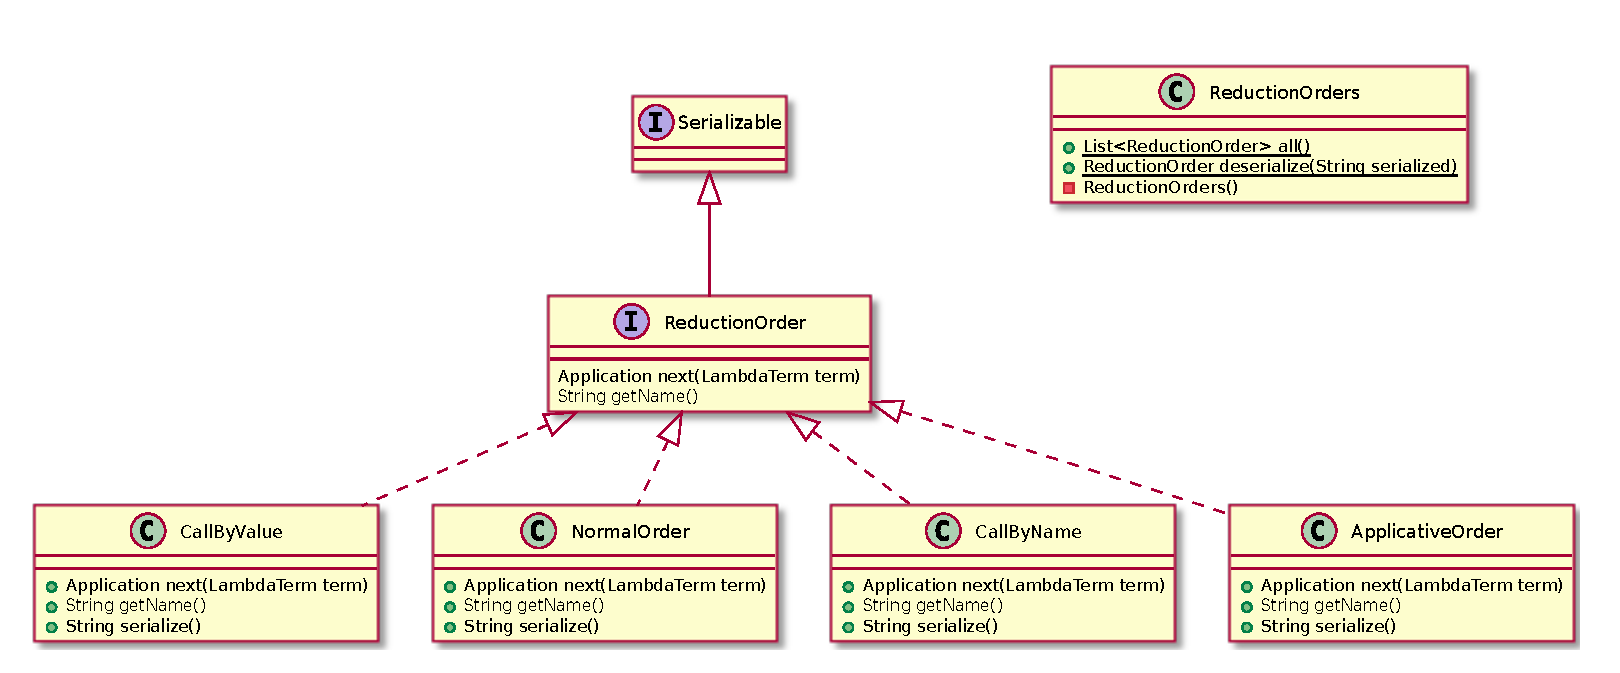
\includegraphics[width=\textwidth]{packageDiagrams/reductionPackage}
\end{figure}
